\documentclass[1p]{elsarticle_modified}
%\bibliographystyle{elsarticle-num}

%\usepackage[colorlinks]{hyperref}
%\usepackage{abbrmath_seonhwa} %\Abb, \Ascr, \Acal ,\Abf, \Afrak
\usepackage{amsfonts}
\usepackage{amssymb}
\usepackage{amsmath}
\usepackage{amsthm}
\usepackage{scalefnt}
\usepackage{amsbsy}
\usepackage{kotex}
\usepackage{caption}
\usepackage{subfig}
\usepackage{color}
\usepackage{graphicx}
\usepackage{xcolor} %% white, black, red, green, blue, cyan, magenta, yellow
\usepackage{float}
\usepackage{setspace}
\usepackage{hyperref}

\usepackage{tikz}
\usetikzlibrary{arrows}

\usepackage{multirow}
\usepackage{array} % fixed length table
\usepackage{hhline}

%%%%%%%%%%%%%%%%%%%%%
\makeatletter
\renewcommand*\env@matrix[1][\arraystretch]{%
	\edef\arraystretch{#1}%
	\hskip -\arraycolsep
	\let\@ifnextchar\new@ifnextchar
	\array{*\c@MaxMatrixCols c}}
\makeatother %https://tex.stackexchange.com/questions/14071/how-can-i-increase-the-line-spacing-in-a-matrix
%%%%%%%%%%%%%%%

\usepackage[normalem]{ulem}

\newcommand{\msout}[1]{\ifmmode\text{\sout{\ensuremath{#1}}}\else\sout{#1}\fi}
%SOURCE: \msout is \stkout macro in https://tex.stackexchange.com/questions/20609/strikeout-in-math-mode

\newcommand{\cancel}[1]{
	\ifmmode
	{\color{red}\msout{#1}}
	\else
	{\color{red}\sout{#1}}
	\fi
}

\newcommand{\add}[1]{
	{\color{blue}\uwave{#1}}
}

\newcommand{\replace}[2]{
	\ifmmode
	{\color{red}\msout{#1}}{\color{blue}\uwave{#2}}
	\else
	{\color{red}\sout{#1}}{\color{blue}\uwave{#2}}
	\fi
}

\newcommand{\Sol}{\mathcal{S}} %segment
\newcommand{\D}{D} %diagram
\newcommand{\A}{\mathcal{A}} %arc


%%%%%%%%%%%%%%%%%%%%%%%%%%%%%5 test

\def\sl{\operatorname{\textup{SL}}(2,\Cbb)}
\def\psl{\operatorname{\textup{PSL}}(2,\Cbb)}
\def\quan{\mkern 1mu \triangleright \mkern 1mu}

\theoremstyle{definition}
\newtheorem{thm}{Theorem}[section]
\newtheorem{prop}[thm]{Proposition}
\newtheorem{lem}[thm]{Lemma}
\newtheorem{ques}[thm]{Question}
\newtheorem{cor}[thm]{Corollary}
\newtheorem{defn}[thm]{Definition}
\newtheorem{exam}[thm]{Example}
\newtheorem{rmk}[thm]{Remark}
\newtheorem{alg}[thm]{Algorithm}

\newcommand{\I}{\sqrt{-1}}
\begin{document}

%\begin{frontmatter}
%
%\title{Boundary parabolic representations of knots up to 8 crossings}
%
%%% Group authors per affiliation:
%\author{Yunhi Cho} 
%\address{Department of Mathematics, University of Seoul, Seoul, Korea}
%\ead{yhcho@uos.ac.kr}
%
%
%\author{Seonhwa Kim} %\fnref{s_kim}}
%\address{Center for Geometry and Physics, Institute for Basic Science, Pohang, 37673, Korea}
%\ead{ryeona17@ibs.re.kr}
%
%\author{Hyuk Kim}
%\address{Department of Mathematical Sciences, Seoul National University, Seoul 08826, Korea}
%\ead{hyukkim@snu.ac.kr}
%
%\author{Seokbeom Yoon}
%\address{Department of Mathematical Sciences, Seoul National University, Seoul, 08826,  Korea}
%\ead{sbyoon15@snu.ac.kr}
%
%\begin{abstract}
%We find all boundary parabolic representation of knots up to 8 crossings.
%
%\end{abstract}
%\begin{keyword}
%    \MSC[2010] 57M25 
%\end{keyword}
%
%\end{frontmatter}

%\linenumbers
%\tableofcontents
%
\newcommand\colored[1]{\textcolor{white}{\rule[-0.35ex]{0.8em}{1.4ex}}\kern-0.8em\color{red} #1}%
%\newcommand\colored[1]{\textcolor{white}{ #1}\kern-2.17ex	\textcolor{white}{ #1}\kern-1.81ex	\textcolor{white}{ #1}\kern-2.15ex\color{red}#1	}

{\Large $\underline{12n_{0712}~(K12n_{0712})}$}

\setlength{\tabcolsep}{10pt}
\renewcommand{\arraystretch}{1.6}
\vspace{1cm}\begin{tabular}{m{100pt}>{\centering\arraybackslash}m{274pt}}
\multirow{5}{120pt}{
	\centering
	\includegraphics[width=112pt]{../../../GIT/diagram.site/Diagrams/png/2801_12n_0712.png}\\
\ \ \ A knot diagram\footnotemark}&
\allowdisplaybreaks
\textbf{Linearized knot diagam} \\
\cline{2-2}
 &
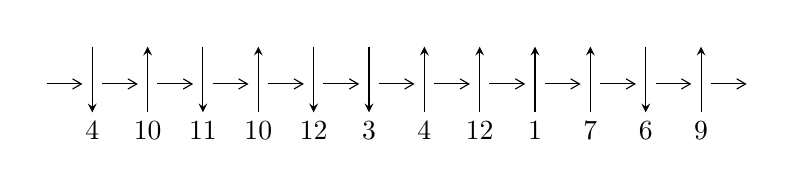
\begin{tikzpicture}[x=20pt, y=17pt]
	% nodes
	\node (C0) at (0, 0) {};
	\node (C1) at (1, 0) {};
	\node (C1U) at (1, +1) {};
	\node (C1D) at (1, -1) {4};

	\node (C2) at (2, 0) {};
	\node (C2U) at (2, +1) {};
	\node (C2D) at (2, -1) {10};

	\node (C3) at (3, 0) {};
	\node (C3U) at (3, +1) {};
	\node (C3D) at (3, -1) {11};

	\node (C4) at (4, 0) {};
	\node (C4U) at (4, +1) {};
	\node (C4D) at (4, -1) {10};

	\node (C5) at (5, 0) {};
	\node (C5U) at (5, +1) {};
	\node (C5D) at (5, -1) {12};

	\node (C6) at (6, 0) {};
	\node (C6U) at (6, +1) {};
	\node (C6D) at (6, -1) {3};

	\node (C7) at (7, 0) {};
	\node (C7U) at (7, +1) {};
	\node (C7D) at (7, -1) {4};

	\node (C8) at (8, 0) {};
	\node (C8U) at (8, +1) {};
	\node (C8D) at (8, -1) {12};

	\node (C9) at (9, 0) {};
	\node (C9U) at (9, +1) {};
	\node (C9D) at (9, -1) {1};

	\node (C10) at (10, 0) {};
	\node (C10U) at (10, +1) {};
	\node (C10D) at (10, -1) {7};

	\node (C11) at (11, 0) {};
	\node (C11U) at (11, +1) {};
	\node (C11D) at (11, -1) {6};

	\node (C12) at (12, 0) {};
	\node (C12U) at (12, +1) {};
	\node (C12D) at (12, -1) {9};
	\node (C13) at (13, 0) {};

	% arrows
	\draw[->,>={angle 60}]
	(C0) edge (C1) (C1) edge (C2) (C2) edge (C3) (C3) edge (C4) (C4) edge (C5) (C5) edge (C6) (C6) edge (C7) (C7) edge (C8) (C8) edge (C9) (C9) edge (C10) (C10) edge (C11) (C11) edge (C12) (C12) edge (C13) ;	\draw[->,>=stealth]
	(C1U) edge (C1D) (C2D) edge (C2U) (C3U) edge (C3D) (C4D) edge (C4U) (C5U) edge (C5D) (C6U) edge (C6D) (C7D) edge (C7U) (C8D) edge (C8U) (C9D) edge (C9U) (C10D) edge (C10U) (C11U) edge (C11D) (C12D) edge (C12U) ;
	\end{tikzpicture} \\
\hhline{~~} \\& 
\textbf{Solving Sequence} \\ \cline{2-2} 
 &
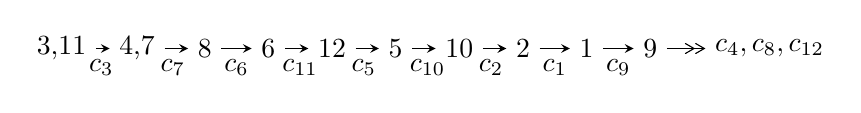
\begin{tikzpicture}[x=23pt, y=7pt]
	% node
	\node (A0) at (-1/8, 0) {3,11};
	\node (A1) at (17/16, 0) {4,7};
	\node (A2) at (17/8, 0) {8};
	\node (A3) at (25/8, 0) {6};
	\node (A4) at (33/8, 0) {12};
	\node (A5) at (41/8, 0) {5};
	\node (A6) at (49/8, 0) {10};
	\node (A7) at (57/8, 0) {2};
	\node (A8) at (65/8, 0) {1};
	\node (A9) at (73/8, 0) {9};
	\node (C1) at (1/2, -1) {$c_{3}$};
	\node (C2) at (13/8, -1) {$c_{7}$};
	\node (C3) at (21/8, -1) {$c_{6}$};
	\node (C4) at (29/8, -1) {$c_{11}$};
	\node (C5) at (37/8, -1) {$c_{5}$};
	\node (C6) at (45/8, -1) {$c_{10}$};
	\node (C7) at (53/8, -1) {$c_{2}$};
	\node (C8) at (61/8, -1) {$c_{1}$};
	\node (C9) at (69/8, -1) {$c_{9}$};
	\node (A10) at (11, 0) {$c_{4},c_{8},c_{12}$};

	% edge
	\draw[->,>=stealth]	
	(A0) edge (A1) (A1) edge (A2) (A2) edge (A3) (A3) edge (A4) (A4) edge (A5) (A5) edge (A6) (A6) edge (A7) (A7) edge (A8) (A8) edge (A9) ;
	\draw[->>,>={angle 60}]	
	(A9) edge (A10);
\end{tikzpicture} \\ 

\end{tabular} \\

\footnotetext{
The image of knot diagram is generated by the software ``\textbf{Draw programme}" developed by Andrew Bartholomew(\url{http://www.layer8.co.uk/maths/draw/index.htm\#Running-draw}), where we modified some parts for our purpose(\url{https://github.com/CATsTAILs/LinksPainter}).
}\phantom \\ \newline 
\centering \textbf{Ideals for irreducible components\footnotemark of $X_{\text{par}}$} 
 
\begin{align*}
I^u_{1}&=\langle 
7.16436\times10^{249} u^{75}+2.01743\times10^{250} u^{74}+\cdots+3.69252\times10^{250} b-9.34607\times10^{250},\\
\phantom{I^u_{1}}&\phantom{= \langle  }8.19251\times10^{249} u^{75}+2.51790\times10^{250} u^{74}+\cdots+3.69252\times10^{250} a-2.00281\times10^{251},\;u^{76}+3 u^{75}+\cdots-40 u-8\rangle \\
I^u_{2}&=\langle 
-6040320 u^{16}+4996901 u^{15}+\cdots+9996367 b-9918960,\\
\phantom{I^u_{2}}&\phantom{= \langle  }1258838 u^{16}-20888294 u^{15}+\cdots+9996367 a+50252931,\;u^{17}+3 u^{15}+\cdots+u-1\rangle \\
\\
\end{align*}
\raggedright * 2 irreducible components of $\dim_{\mathbb{C}}=0$, with total 93 representations.\\
\footnotetext{All coefficients of polynomials are rational numbers. But the coefficients are sometimes approximated in decimal forms when there is not enough margin.}
\newpage
\renewcommand{\arraystretch}{1}
\centering \section*{I. $I^u_{1}= \langle 7.16\times10^{249} u^{75}+2.02\times10^{250} u^{74}+\cdots+3.69\times10^{250} b-9.35\times10^{250},\;8.19\times10^{249} u^{75}+2.52\times10^{250} u^{74}+\cdots+3.69\times10^{250} a-2.00\times10^{251},\;u^{76}+3 u^{75}+\cdots-40 u-8 \rangle$}
\flushleft \textbf{(i) Arc colorings}\\
\begin{tabular}{m{7pt} m{180pt} m{7pt} m{180pt} }
\flushright $a_{3}=$&$\begin{pmatrix}1\\0\end{pmatrix}$ \\
\flushright $a_{11}=$&$\begin{pmatrix}0\\u\end{pmatrix}$ \\
\flushright $a_{4}=$&$\begin{pmatrix}1\\u^2\end{pmatrix}$ \\
\flushright $a_{7}=$&$\begin{pmatrix}-0.221867 u^{75}-0.681890 u^{74}+\cdots+21.9887 u+5.42396\\-0.194023 u^{75}-0.546355 u^{74}+\cdots+17.3170 u+2.53108\end{pmatrix}$ \\
\flushright $a_{8}=$&$\begin{pmatrix}-0.444577 u^{75}-1.31396 u^{74}+\cdots+41.7321 u+8.08534\\-0.189585 u^{75}-0.533144 u^{74}+\cdots+16.9775 u+2.81951\end{pmatrix}$ \\
\flushright $a_{6}=$&$\begin{pmatrix}-0.415891 u^{75}-1.22824 u^{74}+\cdots+39.3057 u+7.95504\\-0.194023 u^{75}-0.546355 u^{74}+\cdots+17.3170 u+2.53108\end{pmatrix}$ \\
\flushright $a_{12}=$&$\begin{pmatrix}-0.0622434 u^{75}-0.0455723 u^{74}+\cdots-33.2165 u-8.05740\\-0.0439022 u^{75}-0.116446 u^{74}+\cdots+1.87201 u+1.57885\end{pmatrix}$ \\
\flushright $a_{5}=$&$\begin{pmatrix}0.651878 u^{75}+1.92544 u^{74}+\cdots-51.0468 u-2.30852\\-0.0179655 u^{75}-0.0546002 u^{74}+\cdots+3.42243 u+2.09091\end{pmatrix}$ \\
\flushright $a_{10}=$&$\begin{pmatrix}-0.0294076 u^{75}+0.0381562 u^{74}+\cdots-28.1824 u-9.55530\\0.0110664 u^{75}+0.0327171 u^{74}+\cdots-4.90611 u-0.0809515\end{pmatrix}$ \\
\flushright $a_{2}=$&$\begin{pmatrix}-0.317501 u^{75}-0.942464 u^{74}+\cdots+28.4231 u+3.04039\\0.0616004 u^{75}+0.175235 u^{74}+\cdots-5.56085 u-2.01059\end{pmatrix}$ \\
\flushright $a_{1}=$&$\begin{pmatrix}-0.299536 u^{75}-0.887864 u^{74}+\cdots+25.0007 u+0.949486\\0.0645846 u^{75}+0.181799 u^{74}+\cdots-5.38898 u-2.00496\end{pmatrix}$ \\
\flushright $a_{9}=$&$\begin{pmatrix}-0.442676 u^{75}-1.15751 u^{74}+\cdots+2.36444 u-4.96056\\-0.0699751 u^{75}-0.183763 u^{74}+\cdots+4.34691 u+0.572363\end{pmatrix}$\\&\end{tabular}
\flushleft \textbf{(ii) Obstruction class $= -1$}\\~\\
\flushleft \textbf{(iii) Cusp Shapes $= 0.982921 u^{75}+2.54015 u^{74}+\cdots-83.5290 u-1.53183$}\\~\\
\newpage\renewcommand{\arraystretch}{1}
\flushleft \textbf{(iv) u-Polynomials at the component}\newline \\
\begin{tabular}{m{50pt}|m{274pt}}
Crossings & \hspace{64pt}u-Polynomials at each crossing \\
\hline $$\begin{aligned}c_{1}\end{aligned}$$&$\begin{aligned}
&u^{76}+5 u^{75}+\cdots+14139 u+307
\end{aligned}$\\
\hline $$\begin{aligned}c_{2}\end{aligned}$$&$\begin{aligned}
&u^{76}+16 u^{74}+\cdots-417 u+9
\end{aligned}$\\
\hline $$\begin{aligned}c_{3}\end{aligned}$$&$\begin{aligned}
&u^{76}-3 u^{75}+\cdots+40 u-8
\end{aligned}$\\
\hline $$\begin{aligned}c_{4}\end{aligned}$$&$\begin{aligned}
&u^{76}+25 u^{74}+\cdots-40832 u-9472
\end{aligned}$\\
\hline $$\begin{aligned}c_{5},c_{11}\end{aligned}$$&$\begin{aligned}
&u^{76}+21 u^{74}+\cdots-7422 u-4041
\end{aligned}$\\
\hline $$\begin{aligned}c_{6}\end{aligned}$$&$\begin{aligned}
&u^{76}+5 u^{75}+\cdots-14 u+1
\end{aligned}$\\
\hline $$\begin{aligned}c_{7}\end{aligned}$$&$\begin{aligned}
&u^{76}+u^{75}+\cdots+280 u-19
\end{aligned}$\\
\hline $$\begin{aligned}c_{8},c_{9},c_{12}\end{aligned}$$&$\begin{aligned}
&u^{76}-32 u^{74}+\cdots-141 u+19
\end{aligned}$\\
\hline $$\begin{aligned}c_{10}\end{aligned}$$&$\begin{aligned}
&u^{76}-4 u^{75}+\cdots+100 u-1
\end{aligned}$\\
\hline
\end{tabular}\\~\\
\newpage\renewcommand{\arraystretch}{1}
\flushleft \textbf{(v) Riley Polynomials at the component}\newline \\
\begin{tabular}{m{50pt}|m{274pt}}
Crossings & \hspace{64pt}Riley Polynomials at each crossing \\
\hline $$\begin{aligned}c_{1}\end{aligned}$$&$\begin{aligned}
&y^{76}-57 y^{75}+\cdots-374836851 y+94249
\end{aligned}$\\
\hline $$\begin{aligned}c_{2}\end{aligned}$$&$\begin{aligned}
&y^{76}+32 y^{75}+\cdots-151605 y+81
\end{aligned}$\\
\hline $$\begin{aligned}c_{3}\end{aligned}$$&$\begin{aligned}
&y^{76}+13 y^{75}+\cdots+1568 y+64
\end{aligned}$\\
\hline $$\begin{aligned}c_{4}\end{aligned}$$&$\begin{aligned}
&y^{76}+50 y^{75}+\cdots+4136583168 y+89718784
\end{aligned}$\\
\hline $$\begin{aligned}c_{5},c_{11}\end{aligned}$$&$\begin{aligned}
&y^{76}+42 y^{75}+\cdots+335290680 y+16329681
\end{aligned}$\\
\hline $$\begin{aligned}c_{6}\end{aligned}$$&$\begin{aligned}
&y^{76}+9 y^{75}+\cdots-22 y+1
\end{aligned}$\\
\hline $$\begin{aligned}c_{7}\end{aligned}$$&$\begin{aligned}
&y^{76}+17 y^{75}+\cdots-28924 y+361
\end{aligned}$\\
\hline $$\begin{aligned}c_{8},c_{9},c_{12}\end{aligned}$$&$\begin{aligned}
&y^{76}-64 y^{75}+\cdots+5199 y+361
\end{aligned}$\\
\hline $$\begin{aligned}c_{10}\end{aligned}$$&$\begin{aligned}
&y^{76}+10 y^{75}+\cdots-8956 y+1
\end{aligned}$\\
\hline
\end{tabular}\\~\\
\newpage\flushleft \textbf{(vi) Complex Volumes and Cusp Shapes}
$$\begin{array}{c|c|c}  
\text{Solutions to }I^u_{1}& \I (\text{vol} + \sqrt{-1}CS) & \text{Cusp shape}\\
 \hline 
\begin{aligned}
u &= -0.988673 + 0.157879 I \\
a &= \phantom{-}0.210479 - 0.611484 I \\
b &= -0.77585 + 1.64641 I\end{aligned}
 & \phantom{-}0.29226 + 5.94254 I & \phantom{-0.000000 } 0 \\ \hline\begin{aligned}
u &= -0.988673 - 0.157879 I \\
a &= \phantom{-}0.210479 + 0.611484 I \\
b &= -0.77585 - 1.64641 I\end{aligned}
 & \phantom{-}0.29226 - 5.94254 I & \phantom{-0.000000 } 0 \\ \hline\begin{aligned}
u &= -0.856136 + 0.519729 I \\
a &= \phantom{-}0.138708 + 0.873657 I \\
b &= -0.09153 - 1.49560 I\end{aligned}
 & \phantom{-}0.21542 + 4.69032 I & \phantom{-0.000000 } 0 \\ \hline\begin{aligned}
u &= -0.856136 - 0.519729 I \\
a &= \phantom{-}0.138708 - 0.873657 I \\
b &= -0.09153 + 1.49560 I\end{aligned}
 & \phantom{-}0.21542 - 4.69032 I & \phantom{-0.000000 } 0 \\ \hline\begin{aligned}
u &= -0.791352 + 0.617036 I \\
a &= \phantom{-}0.037093 + 1.016310 I \\
b &= \phantom{-}0.642295 - 1.104590 I\end{aligned}
 & \phantom{-}0.55399 + 4.14989 I & \phantom{-0.000000 } 0 \\ \hline\begin{aligned}
u &= -0.791352 - 0.617036 I \\
a &= \phantom{-}0.037093 - 1.016310 I \\
b &= \phantom{-}0.642295 + 1.104590 I\end{aligned}
 & \phantom{-}0.55399 - 4.14989 I & \phantom{-0.000000 } 0 \\ \hline\begin{aligned}
u &= \phantom{-}0.274686 + 0.996744 I \\
a &= -0.488851 - 0.812735 I \\
b &= -0.457165 + 0.633310 I\end{aligned}
 & \phantom{-}6.38323 - 2.69065 I & \phantom{-0.000000 } 0 \\ \hline\begin{aligned}
u &= \phantom{-}0.274686 - 0.996744 I \\
a &= -0.488851 + 0.812735 I \\
b &= -0.457165 - 0.633310 I\end{aligned}
 & \phantom{-}6.38323 + 2.69065 I & \phantom{-0.000000 } 0 \\ \hline\begin{aligned}
u &= -0.836004 + 0.659794 I \\
a &= \phantom{-}0.06104 - 1.56008 I \\
b &= -0.880984 + 0.616441 I\end{aligned}
 & -6.58488 + 4.99744 I & \phantom{-0.000000 } 0 \\ \hline\begin{aligned}
u &= -0.836004 - 0.659794 I \\
a &= \phantom{-}0.06104 + 1.56008 I \\
b &= -0.880984 - 0.616441 I\end{aligned}
 & -6.58488 - 4.99744 I & \phantom{-0.000000 } 0\\
 \hline 
 \end{array}$$\newpage$$\begin{array}{c|c|c}  
\text{Solutions to }I^u_{1}& \I (\text{vol} + \sqrt{-1}CS) & \text{Cusp shape}\\
 \hline 
\begin{aligned}
u &= -0.347092 + 0.856959 I \\
a &= \phantom{-}1.28732 + 1.16537 I \\
b &= \phantom{-}0.451088 - 0.953532 I\end{aligned}
 & \phantom{-}3.58206 + 8.75485 I & \phantom{-}8.32937 - 7.77105 I \\ \hline\begin{aligned}
u &= -0.347092 - 0.856959 I \\
a &= \phantom{-}1.28732 - 1.16537 I \\
b &= \phantom{-}0.451088 + 0.953532 I\end{aligned}
 & \phantom{-}3.58206 - 8.75485 I & \phantom{-}8.32937 + 7.77105 I \\ \hline\begin{aligned}
u &= \phantom{-}0.878556 + 0.200637 I \\
a &= \phantom{-}0.238847 - 0.740853 I \\
b &= -0.40970 + 1.78620 I\end{aligned}
 & -3.57909 + 0.60336 I & -2.63945 + 2.67457 I \\ \hline\begin{aligned}
u &= \phantom{-}0.878556 - 0.200637 I \\
a &= \phantom{-}0.238847 + 0.740853 I \\
b &= -0.40970 - 1.78620 I\end{aligned}
 & -3.57909 - 0.60336 I & -2.63945 - 2.67457 I \\ \hline\begin{aligned}
u &= \phantom{-}0.699124 + 0.554855 I \\
a &= \phantom{-}0.15882 + 1.84694 I \\
b &= -0.853372 - 0.594063 I\end{aligned}
 & -2.66450 + 0.00138 I & \phantom{-}0.99118 + 2.31235 I \\ \hline\begin{aligned}
u &= \phantom{-}0.699124 - 0.554855 I \\
a &= \phantom{-}0.15882 - 1.84694 I \\
b &= -0.853372 + 0.594063 I\end{aligned}
 & -2.66450 - 0.00138 I & \phantom{-}0.99118 - 2.31235 I \\ \hline\begin{aligned}
u &= \phantom{-}0.644694 + 0.906666 I \\
a &= -0.091006 - 1.240470 I \\
b &= \phantom{-}1.00187 + 1.51947 I\end{aligned}
 & \phantom{-}9.65535 - 5.48513 I & \phantom{-0.000000 } 0 \\ \hline\begin{aligned}
u &= \phantom{-}0.644694 - 0.906666 I \\
a &= -0.091006 + 1.240470 I \\
b &= \phantom{-}1.00187 - 1.51947 I\end{aligned}
 & \phantom{-}9.65535 + 5.48513 I & \phantom{-0.000000 } 0 \\ \hline\begin{aligned}
u &= \phantom{-}0.394933 + 0.781994 I \\
a &= \phantom{-}1.36967 - 1.13329 I \\
b &= \phantom{-}0.361605 + 0.847407 I\end{aligned}
 & -1.42075 - 4.05339 I & \phantom{-}4.25074 + 6.84714 I \\ \hline\begin{aligned}
u &= \phantom{-}0.394933 - 0.781994 I \\
a &= \phantom{-}1.36967 + 1.13329 I \\
b &= \phantom{-}0.361605 - 0.847407 I\end{aligned}
 & -1.42075 + 4.05339 I & \phantom{-}4.25074 - 6.84714 I\\
 \hline 
 \end{array}$$\newpage$$\begin{array}{c|c|c}  
\text{Solutions to }I^u_{1}& \I (\text{vol} + \sqrt{-1}CS) & \text{Cusp shape}\\
 \hline 
\begin{aligned}
u &= \phantom{-}0.723650 + 0.459547 I \\
a &= \phantom{-}0.035116 - 0.774350 I \\
b &= \phantom{-}0.655940 + 0.546441 I\end{aligned}
 & -1.18749 - 1.04073 I & -2.87515 + 1.88476 I \\ \hline\begin{aligned}
u &= \phantom{-}0.723650 - 0.459547 I \\
a &= \phantom{-}0.035116 + 0.774350 I \\
b &= \phantom{-}0.655940 - 0.546441 I\end{aligned}
 & -1.18749 + 1.04073 I & -2.87515 - 1.88476 I \\ \hline\begin{aligned}
u &= \phantom{-}0.802133 + 0.883320 I \\
a &= -0.451106 - 0.482056 I \\
b &= -0.418768 - 0.183701 I\end{aligned}
 & \phantom{-}6.65595 - 3.01746 I & \phantom{-0.000000 } 0 \\ \hline\begin{aligned}
u &= \phantom{-}0.802133 - 0.883320 I \\
a &= -0.451106 + 0.482056 I \\
b &= -0.418768 + 0.183701 I\end{aligned}
 & \phantom{-}6.65595 + 3.01746 I & \phantom{-0.000000 } 0 \\ \hline\begin{aligned}
u &= \phantom{-}0.925583 + 0.764929 I \\
a &= \phantom{-}0.027137 + 1.376180 I \\
b &= -0.895559 - 0.641011 I\end{aligned}
 & -2.50803 - 9.92376 I & \phantom{-0.000000 } 0 \\ \hline\begin{aligned}
u &= \phantom{-}0.925583 - 0.764929 I \\
a &= \phantom{-}0.027137 - 1.376180 I \\
b &= -0.895559 + 0.641011 I\end{aligned}
 & -2.50803 + 9.92376 I & \phantom{-0.000000 } 0 \\ \hline\begin{aligned}
u &= -0.464123 + 0.622645 I \\
a &= \phantom{-}1.42148 + 1.07836 I \\
b &= \phantom{-}0.249050 - 0.626220 I\end{aligned}
 & \phantom{-}1.25423 - 0.69104 I & \phantom{-}7.01445 - 3.43740 I \\ \hline\begin{aligned}
u &= -0.464123 - 0.622645 I \\
a &= \phantom{-}1.42148 - 1.07836 I \\
b &= \phantom{-}0.249050 + 0.626220 I\end{aligned}
 & \phantom{-}1.25423 + 0.69104 I & \phantom{-}7.01445 + 3.43740 I \\ \hline\begin{aligned}
u &= -1.24798\phantom{ +0.000000I} \\
a &= \phantom{-}0.00845205\phantom{ +0.000000I} \\
b &= \phantom{-}0.614730\phantom{ +0.000000I}\end{aligned}
 & \phantom{-}2.40053\phantom{ +0.000000I} & \phantom{-0.000000 } 0 \\ \hline\begin{aligned}
u &= -0.245836 + 0.608610 I \\
a &= -1.01333 + 1.76814 I \\
b &= -0.189251 - 0.380413 I\end{aligned}
 & \phantom{-}1.92153 + 0.94962 I & -2.98543 - 0.44875 I\\
 \hline 
 \end{array}$$\newpage$$\begin{array}{c|c|c}  
\text{Solutions to }I^u_{1}& \I (\text{vol} + \sqrt{-1}CS) & \text{Cusp shape}\\
 \hline 
\begin{aligned}
u &= -0.245836 - 0.608610 I \\
a &= -1.01333 - 1.76814 I \\
b &= -0.189251 + 0.380413 I\end{aligned}
 & \phantom{-}1.92153 - 0.94962 I & -2.98543 + 0.44875 I \\ \hline\begin{aligned}
u &= \phantom{-}0.079389 + 0.643195 I \\
a &= \phantom{-}1.88748 - 1.54979 I \\
b &= -0.427883 + 0.986505 I\end{aligned}
 & \phantom{-}9.02338 + 2.28669 I & \phantom{-}0.66173 + 6.35182 I \\ \hline\begin{aligned}
u &= \phantom{-}0.079389 - 0.643195 I \\
a &= \phantom{-}1.88748 + 1.54979 I \\
b &= -0.427883 - 0.986505 I\end{aligned}
 & \phantom{-}9.02338 - 2.28669 I & \phantom{-}0.66173 - 6.35182 I \\ \hline\begin{aligned}
u &= \phantom{-}0.659231 + 1.237980 I \\
a &= -0.029277 + 0.560989 I \\
b &= -0.983298 - 0.893974 I\end{aligned}
 & \phantom{-}8.19481 - 3.33586 I & \phantom{-0.000000 } 0 \\ \hline\begin{aligned}
u &= \phantom{-}0.659231 - 1.237980 I \\
a &= -0.029277 - 0.560989 I \\
b &= -0.983298 + 0.893974 I\end{aligned}
 & \phantom{-}8.19481 + 3.33586 I & \phantom{-0.000000 } 0 \\ \hline\begin{aligned}
u &= -0.98850 + 1.01710 I \\
a &= -0.138103 + 0.999293 I \\
b &= \phantom{-}1.06198 - 1.21767 I\end{aligned}
 & -0.46066 + 6.48918 I & \phantom{-0.000000 } 0 \\ \hline\begin{aligned}
u &= -0.98850 - 1.01710 I \\
a &= -0.138103 - 0.999293 I \\
b &= \phantom{-}1.06198 + 1.21767 I\end{aligned}
 & -0.46066 - 6.48918 I & \phantom{-0.000000 } 0 \\ \hline\begin{aligned}
u &= -0.328939 + 0.463886 I \\
a &= \phantom{-}1.55302 + 0.64027 I \\
b &= -0.053887 - 0.497588 I\end{aligned}
 & \phantom{-}1.328470 - 0.474798 I & \phantom{-}6.36942 - 0.30577 I \\ \hline\begin{aligned}
u &= -0.328939 - 0.463886 I \\
a &= \phantom{-}1.55302 - 0.64027 I \\
b &= -0.053887 + 0.497588 I\end{aligned}
 & \phantom{-}1.328470 + 0.474798 I & \phantom{-}6.36942 + 0.30577 I \\ \hline\begin{aligned}
u &= \phantom{-}0.534569 + 0.150336 I \\
a &= -0.376119 - 1.361820 I \\
b &= \phantom{-}1.31070 + 0.63115 I\end{aligned}
 & -2.20215 - 2.11422 I & -3.95825 + 2.02066 I\\
 \hline 
 \end{array}$$\newpage$$\begin{array}{c|c|c}  
\text{Solutions to }I^u_{1}& \I (\text{vol} + \sqrt{-1}CS) & \text{Cusp shape}\\
 \hline 
\begin{aligned}
u &= \phantom{-}0.534569 - 0.150336 I \\
a &= -0.376119 + 1.361820 I \\
b &= \phantom{-}1.31070 - 0.63115 I\end{aligned}
 & -2.20215 + 2.11422 I & -3.95825 - 2.02066 I \\ \hline\begin{aligned}
u &= \phantom{-}0.526151\phantom{ +0.000000I} \\
a &= \phantom{-}4.68059\phantom{ +0.000000I} \\
b &= \phantom{-}0.222446\phantom{ +0.000000I}\end{aligned}
 & \phantom{-}3.74373\phantom{ +0.000000I} & -111.560\phantom{ +0.000000I} \\ \hline\begin{aligned}
u &= -0.97016 + 1.10954 I \\
a &= \phantom{-}0.091135 - 0.575325 I \\
b &= -0.885716 + 1.032580 I\end{aligned}
 & \phantom{-}3.43380 + 4.26674 I & \phantom{-0.000000 } 0 \\ \hline\begin{aligned}
u &= -0.97016 - 1.10954 I \\
a &= \phantom{-}0.091135 + 0.575325 I \\
b &= -0.885716 - 1.032580 I\end{aligned}
 & \phantom{-}3.43380 - 4.26674 I & \phantom{-0.000000 } 0 \\ \hline\begin{aligned}
u &= -0.281385 + 0.377115 I \\
a &= -1.73924 + 1.56042 I \\
b &= -0.465609 + 0.236668 I\end{aligned}
 & \phantom{-}1.70817 + 1.12824 I & \phantom{-}3.87173 - 6.48533 I \\ \hline\begin{aligned}
u &= -0.281385 - 0.377115 I \\
a &= -1.73924 - 1.56042 I \\
b &= -0.465609 - 0.236668 I\end{aligned}
 & \phantom{-}1.70817 - 1.12824 I & \phantom{-}3.87173 + 6.48533 I \\ \hline\begin{aligned}
u &= \phantom{-}0.130457 + 0.443544 I \\
a &= \phantom{-}0.83864 + 1.48325 I \\
b &= \phantom{-}1.53456 - 1.51852 I\end{aligned}
 & \phantom{-}1.75853 - 7.50443 I & \phantom{-}7.50202 + 11.32011 I \\ \hline\begin{aligned}
u &= \phantom{-}0.130457 - 0.443544 I \\
a &= \phantom{-}0.83864 - 1.48325 I \\
b &= \phantom{-}1.53456 + 1.51852 I\end{aligned}
 & \phantom{-}1.75853 + 7.50443 I & \phantom{-}7.50202 - 11.32011 I \\ \hline\begin{aligned}
u &= -0.43167 + 1.47701 I \\
a &= -0.497084 - 0.041859 I \\
b &= \phantom{-}1.065130 + 0.173695 I\end{aligned}
 & -4.34097 + 0.35523 I & \phantom{-0.000000 } 0 \\ \hline\begin{aligned}
u &= -0.43167 - 1.47701 I \\
a &= -0.497084 + 0.041859 I \\
b &= \phantom{-}1.065130 - 0.173695 I\end{aligned}
 & -4.34097 - 0.35523 I & \phantom{-0.000000 } 0\\
 \hline 
 \end{array}$$\newpage$$\begin{array}{c|c|c}  
\text{Solutions to }I^u_{1}& \I (\text{vol} + \sqrt{-1}CS) & \text{Cusp shape}\\
 \hline 
\begin{aligned}
u &= \phantom{-}1.03967 + 1.15434 I \\
a &= -0.175674 - 0.949551 I \\
b &= \phantom{-}1.10780 + 1.18726 I\end{aligned}
 & -3.18134 - 11.88140 I & \phantom{-0.000000 } 0 \\ \hline\begin{aligned}
u &= \phantom{-}1.03967 - 1.15434 I \\
a &= -0.175674 + 0.949551 I \\
b &= \phantom{-}1.10780 - 1.18726 I\end{aligned}
 & -3.18134 + 11.88140 I & \phantom{-0.000000 } 0 \\ \hline\begin{aligned}
u &= -1.07256 + 1.16076 I \\
a &= \phantom{-}0.518563 - 0.163208 I \\
b &= -0.354403 - 0.325175 I\end{aligned}
 & -0.346472 + 1.021960 I & \phantom{-0.000000 } 0 \\ \hline\begin{aligned}
u &= -1.07256 - 1.16076 I \\
a &= \phantom{-}0.518563 + 0.163208 I \\
b &= -0.354403 + 0.325175 I\end{aligned}
 & -0.346472 - 1.021960 I & \phantom{-0.000000 } 0 \\ \hline\begin{aligned}
u &= -0.065520 + 0.389048 I \\
a &= -3.90518 + 0.23427 I \\
b &= -0.663122 - 0.134399 I\end{aligned}
 & \phantom{-}3.88542 + 0.95380 I & -0.53894 + 3.77835 I \\ \hline\begin{aligned}
u &= -0.065520 - 0.389048 I \\
a &= -3.90518 - 0.23427 I \\
b &= -0.663122 + 0.134399 I\end{aligned}
 & \phantom{-}3.88542 - 0.95380 I & -0.53894 - 3.77835 I \\ \hline\begin{aligned}
u &= \phantom{-}0.91249 + 1.33131 I \\
a &= \phantom{-}0.152639 + 0.727902 I \\
b &= -0.806727 - 0.838803 I\end{aligned}
 & \phantom{-}2.28311 - 5.16223 I & \phantom{-0.000000 } 0 \\ \hline\begin{aligned}
u &= \phantom{-}0.91249 - 1.33131 I \\
a &= \phantom{-}0.152639 - 0.727902 I \\
b &= -0.806727 + 0.838803 I\end{aligned}
 & \phantom{-}2.28311 + 5.16223 I & \phantom{-0.000000 } 0 \\ \hline\begin{aligned}
u &= \phantom{-}0.18899 + 1.60874 I \\
a &= -0.579596 + 0.139074 I \\
b &= \phantom{-}1.208120 - 0.259339 I\end{aligned}
 & \phantom{-}0.43258 - 3.98462 I & \phantom{-0.000000 } 0 \\ \hline\begin{aligned}
u &= \phantom{-}0.18899 - 1.60874 I \\
a &= -0.579596 - 0.139074 I \\
b &= \phantom{-}1.208120 + 0.259339 I\end{aligned}
 & \phantom{-}0.43258 + 3.98462 I & \phantom{-0.000000 } 0\\
 \hline 
 \end{array}$$\newpage$$\begin{array}{c|c|c}  
\text{Solutions to }I^u_{1}& \I (\text{vol} + \sqrt{-1}CS) & \text{Cusp shape}\\
 \hline 
\begin{aligned}
u &= -1.03600 + 1.25835 I \\
a &= -0.207314 + 0.919011 I \\
b &= \phantom{-}1.13468 - 1.16952 I\end{aligned}
 & \phantom{-}1.8826 + 16.8363 I & \phantom{-0.000000 } 0 \\ \hline\begin{aligned}
u &= -1.03600 - 1.25835 I \\
a &= -0.207314 - 0.919011 I \\
b &= \phantom{-}1.13468 + 1.16952 I\end{aligned}
 & \phantom{-}1.8826 - 16.8363 I & \phantom{-0.000000 } 0 \\ \hline\begin{aligned}
u &= -0.95108 + 1.32857 I \\
a &= \phantom{-}0.036047 - 0.766370 I \\
b &= -0.884370 + 0.831483 I\end{aligned}
 & \phantom{-}6.15358 + 7.92208 I & \phantom{-0.000000 } 0 \\ \hline\begin{aligned}
u &= -0.95108 - 1.32857 I \\
a &= \phantom{-}0.036047 + 0.766370 I \\
b &= -0.884370 - 0.831483 I\end{aligned}
 & \phantom{-}6.15358 - 7.92208 I & \phantom{-0.000000 } 0 \\ \hline\begin{aligned}
u &= \phantom{-}0.82591 + 1.43030 I \\
a &= -0.368712 - 0.006518 I \\
b &= \phantom{-}0.909492 - 0.149096 I\end{aligned}
 & -0.90960 + 3.32063 I & \phantom{-0.000000 } 0 \\ \hline\begin{aligned}
u &= \phantom{-}0.82591 - 1.43030 I \\
a &= -0.368712 + 0.006518 I \\
b &= \phantom{-}0.909492 + 0.149096 I\end{aligned}
 & -0.90960 - 3.32063 I & \phantom{-0.000000 } 0 \\ \hline\begin{aligned}
u &= -0.196925 + 0.198557 I \\
a &= \phantom{-}0.87584 - 2.14816 I \\
b &= \phantom{-}1.92387 + 1.05055 I\end{aligned}
 & -3.96027 + 2.48444 I & -5.35559 - 12.59159 I \\ \hline\begin{aligned}
u &= -0.196925 - 0.198557 I \\
a &= \phantom{-}0.87584 + 2.14816 I \\
b &= \phantom{-}1.92387 - 1.05055 I\end{aligned}
 & -3.96027 - 2.48444 I & -5.35559 + 12.59159 I \\ \hline\begin{aligned}
u &= \phantom{-}1.27946 + 1.20751 I \\
a &= \phantom{-}0.135069 + 0.566822 I \\
b &= -0.726578 - 1.080900 I\end{aligned}
 & \phantom{-}6.23257 - 5.85237 I & \phantom{-0.000000 } 0 \\ \hline\begin{aligned}
u &= \phantom{-}1.27946 - 1.20751 I \\
a &= \phantom{-}0.135069 - 0.566822 I \\
b &= -0.726578 + 1.080900 I\end{aligned}
 & \phantom{-}6.23257 + 5.85237 I & \phantom{-0.000000 } 0\\
 \hline 
 \end{array}$$\newpage$$\begin{array}{c|c|c}  
\text{Solutions to }I^u_{1}& \I (\text{vol} + \sqrt{-1}CS) & \text{Cusp shape}\\
 \hline 
\begin{aligned}
u &= -0.94793 + 1.50677 I \\
a &= \phantom{-}0.230301 - 0.619665 I \\
b &= -0.682958 + 0.866149 I\end{aligned}
 & \phantom{-}5.82633 + 2.70104 I & \phantom{-0.000000 } 0 \\ \hline\begin{aligned}
u &= -0.94793 - 1.50677 I \\
a &= \phantom{-}0.230301 + 0.619665 I \\
b &= -0.682958 - 0.866149 I\end{aligned}
 & \phantom{-}5.82633 - 2.70104 I & \phantom{-0.000000 } 0 \\ \hline\begin{aligned}
u &= \phantom{-}1.50227 + 0.97016 I \\
a &= \phantom{-}0.381804 + 0.242487 I \\
b &= -0.322820 + 0.301588 I\end{aligned}
 & -4.02902 + 3.33307 I & \phantom{-0.000000 } 0 \\ \hline\begin{aligned}
u &= \phantom{-}1.50227 - 0.97016 I \\
a &= \phantom{-}0.381804 - 0.242487 I \\
b &= -0.322820 - 0.301588 I\end{aligned}
 & -4.02902 - 3.33307 I & \phantom{-0.000000 } 0 \\ \hline\begin{aligned}
u &= -1.83497 + 0.74700 I \\
a &= \phantom{-}0.279823 - 0.271827 I \\
b &= -0.307214 - 0.279280 I\end{aligned}
 & \phantom{-}0.17127 - 7.70833 I & \phantom{-0.000000 } 0 \\ \hline\begin{aligned}
u &= -1.83497 - 0.74700 I \\
a &= \phantom{-}0.279823 + 0.271827 I \\
b &= -0.307214 + 0.279280 I\end{aligned}
 & \phantom{-}0.17127 + 7.70833 I & \phantom{-0.000000 } 0\\
 \hline 
 \end{array}$$\newpage\newpage\renewcommand{\arraystretch}{1}
\centering \section*{II. $I^u_{2}= \langle -6.04\times10^{6} u^{16}+5.00\times10^{6} u^{15}+\cdots+1.00\times10^{7} b-9.92\times10^{6},\;1.26\times10^{6} u^{16}-2.09\times10^{7} u^{15}+\cdots+1.00\times10^{7} a+5.03\times10^{7},\;u^{17}+3 u^{15}+\cdots+u-1 \rangle$}
\flushleft \textbf{(i) Arc colorings}\\
\begin{tabular}{m{7pt} m{180pt} m{7pt} m{180pt} }
\flushright $a_{3}=$&$\begin{pmatrix}1\\0\end{pmatrix}$ \\
\flushright $a_{11}=$&$\begin{pmatrix}0\\u\end{pmatrix}$ \\
\flushright $a_{4}=$&$\begin{pmatrix}1\\u^2\end{pmatrix}$ \\
\flushright $a_{7}=$&$\begin{pmatrix}-0.125930 u^{16}+2.08959 u^{15}+\cdots+10.3993 u-5.02712\\0.604252 u^{16}-0.499872 u^{15}+\cdots-2.52114 u+0.992256\end{pmatrix}$ \\
\flushright $a_{8}=$&$\begin{pmatrix}0.138953 u^{16}+1.97910 u^{15}+\cdots+10.0937 u-6.12445\\0.331276 u^{16}-0.372219 u^{15}+\cdots-2.14577 u+0.881767\end{pmatrix}$ \\
\flushright $a_{6}=$&$\begin{pmatrix}0.478322 u^{16}+1.58972 u^{15}+\cdots+7.87816 u-4.03486\\0.604252 u^{16}-0.499872 u^{15}+\cdots-2.52114 u+0.992256\end{pmatrix}$ \\
\flushright $a_{12}=$&$\begin{pmatrix}2.93753 u^{16}-0.213439 u^{15}+\cdots-8.94162 u-5.24626\\-1.08959 u^{16}-0.339369 u^{15}+\cdots+0.901190 u+1.12593\end{pmatrix}$ \\
\flushright $a_{5}=$&$\begin{pmatrix}6.72458 u^{16}-0.347814 u^{15}+\cdots-15.9518 u+7.15302\\-0.0964454 u^{16}+0.0683699 u^{15}+\cdots+1.11139 u-0.589717\end{pmatrix}$ \\
\flushright $a_{10}=$&$\begin{pmatrix}5.12838 u^{16}+0.385878 u^{15}+\cdots-9.07212 u-7.23639\\-1.10126 u^{16}-0.259949 u^{15}+\cdots+1.22931 u+0.864200\end{pmatrix}$ \\
\flushright $a_{2}=$&$\begin{pmatrix}-1.44840 u^{16}-0.264495 u^{15}+\cdots+4.16177 u-1.79318\\0.915875 u^{16}+0.244253 u^{15}+\cdots-2.29530 u+0.325222\end{pmatrix}$ \\
\flushright $a_{1}=$&$\begin{pmatrix}-1.35195 u^{16}-0.332865 u^{15}+\cdots+3.05037 u-1.20347\\0.981428 u^{16}+0.333098 u^{15}+\cdots-2.13048 u+0.256852\end{pmatrix}$ \\
\flushright $a_{9}=$&$\begin{pmatrix}0.0890174 u^{16}-0.254122 u^{15}+\cdots+1.05583 u-5.67538\\0.942381 u^{16}+0.210599 u^{15}+\cdots-2.25734 u+0.290593\end{pmatrix}$\\&\end{tabular}
\flushleft \textbf{(ii) Obstruction class $= 1$}\\~\\
\flushleft \textbf{(iii) Cusp Shapes $= \frac{23991057}{9996367} u^{16}+\frac{18751596}{9996367} u^{15}+\cdots+\frac{16790502}{9996367} u+\frac{371933198}{9996367}$}\\~\\
\newpage\renewcommand{\arraystretch}{1}
\flushleft \textbf{(iv) u-Polynomials at the component}\newline \\
\begin{tabular}{m{50pt}|m{274pt}}
Crossings & \hspace{64pt}u-Polynomials at each crossing \\
\hline $$\begin{aligned}c_{1}\end{aligned}$$&$\begin{aligned}
&u^{17}-8 u^{16}+\cdots-7 u+1
\end{aligned}$\\
\hline $$\begin{aligned}c_{2}\end{aligned}$$&$\begin{aligned}
&u^{17}- u^{16}+\cdots+85 u-11
\end{aligned}$\\
\hline $$\begin{aligned}c_{3}\end{aligned}$$&$\begin{aligned}
&u^{17}+3 u^{15}+\cdots+u-1
\end{aligned}$\\
\hline $$\begin{aligned}c_{4}\end{aligned}$$&$\begin{aligned}
&u^{17}- u^{16}+\cdots- u-1
\end{aligned}$\\
\hline $$\begin{aligned}c_{5}\end{aligned}$$&$\begin{aligned}
&u^{17}- u^{16}+\cdots-8 u-5
\end{aligned}$\\
\hline $$\begin{aligned}c_{6}\end{aligned}$$&$\begin{aligned}
&u^{17}+3 u^{15}+\cdots+6 u+1
\end{aligned}$\\
\hline $$\begin{aligned}c_{7}\end{aligned}$$&$\begin{aligned}
&u^{17}+4 u^{16}+\cdots+6 u-5
\end{aligned}$\\
\hline $$\begin{aligned}c_{8},c_{9}\end{aligned}$$&$\begin{aligned}
&u^{17}- u^{16}+\cdots-3 u+1
\end{aligned}$\\
\hline $$\begin{aligned}c_{10}\end{aligned}$$&$\begin{aligned}
&u^{17}+3 u^{16}+\cdots+3 u^2+1
\end{aligned}$\\
\hline $$\begin{aligned}c_{11}\end{aligned}$$&$\begin{aligned}
&u^{17}+u^{16}+\cdots-8 u+5
\end{aligned}$\\
\hline $$\begin{aligned}c_{12}\end{aligned}$$&$\begin{aligned}
&u^{17}+u^{16}+\cdots-3 u-1
\end{aligned}$\\
\hline
\end{tabular}\\~\\
\newpage\renewcommand{\arraystretch}{1}
\flushleft \textbf{(v) Riley Polynomials at the component}\newline \\
\begin{tabular}{m{50pt}|m{274pt}}
Crossings & \hspace{64pt}Riley Polynomials at each crossing \\
\hline $$\begin{aligned}c_{1}\end{aligned}$$&$\begin{aligned}
&y^{17}-14 y^{15}+\cdots+5 y-1
\end{aligned}$\\
\hline $$\begin{aligned}c_{2}\end{aligned}$$&$\begin{aligned}
&y^{17}+9 y^{16}+\cdots+2407 y-121
\end{aligned}$\\
\hline $$\begin{aligned}c_{3}\end{aligned}$$&$\begin{aligned}
&y^{17}+6 y^{16}+\cdots-9 y-1
\end{aligned}$\\
\hline $$\begin{aligned}c_{4}\end{aligned}$$&$\begin{aligned}
&y^{17}- y^{16}+\cdots+15 y-1
\end{aligned}$\\
\hline $$\begin{aligned}c_{5},c_{11}\end{aligned}$$&$\begin{aligned}
&y^{17}+11 y^{16}+\cdots-186 y-25
\end{aligned}$\\
\hline $$\begin{aligned}c_{6}\end{aligned}$$&$\begin{aligned}
&y^{17}+6 y^{16}+\cdots+20 y-1
\end{aligned}$\\
\hline $$\begin{aligned}c_{7}\end{aligned}$$&$\begin{aligned}
&y^{17}+6 y^{16}+\cdots+46 y-25
\end{aligned}$\\
\hline $$\begin{aligned}c_{8},c_{9},c_{12}\end{aligned}$$&$\begin{aligned}
&y^{17}-19 y^{16}+\cdots+23 y-1
\end{aligned}$\\
\hline $$\begin{aligned}c_{10}\end{aligned}$$&$\begin{aligned}
&y^{17}- y^{16}+\cdots-6 y-1
\end{aligned}$\\
\hline
\end{tabular}\\~\\
\newpage\flushleft \textbf{(vi) Complex Volumes and Cusp Shapes}
$$\begin{array}{c|c|c}  
\text{Solutions to }I^u_{2}& \I (\text{vol} + \sqrt{-1}CS) & \text{Cusp shape}\\
 \hline 
\begin{aligned}
u &= \phantom{-}0.972003 + 0.212018 I \\
a &= -0.488289 - 0.271559 I \\
b &= \phantom{-}0.336060 + 1.308020 I\end{aligned}
 & \phantom{-}1.01866 + 6.81301 I & \phantom{-}4.54269 - 5.97212 I \\ \hline\begin{aligned}
u &= \phantom{-}0.972003 - 0.212018 I \\
a &= -0.488289 + 0.271559 I \\
b &= \phantom{-}0.336060 - 1.308020 I\end{aligned}
 & \phantom{-}1.01866 - 6.81301 I & \phantom{-}4.54269 + 5.97212 I \\ \hline\begin{aligned}
u &= \phantom{-}0.192968 + 1.105900 I \\
a &= -0.631721 + 0.168013 I \\
b &= \phantom{-}0.883233 + 0.254108 I\end{aligned}
 & -0.82435 - 2.10930 I & \phantom{-}2.15224 + 0.70653 I \\ \hline\begin{aligned}
u &= \phantom{-}0.192968 - 1.105900 I \\
a &= -0.631721 - 0.168013 I \\
b &= \phantom{-}0.883233 - 0.254108 I\end{aligned}
 & -0.82435 + 2.10930 I & \phantom{-}2.15224 - 0.70653 I \\ \hline\begin{aligned}
u &= -0.506977 + 0.637369 I \\
a &= -0.605526 + 0.069770 I \\
b &= \phantom{-}1.09502 - 0.93131 I\end{aligned}
 & -3.76213 - 1.93723 I & \phantom{-}0.705082 + 0.084395 I \\ \hline\begin{aligned}
u &= -0.506977 - 0.637369 I \\
a &= -0.605526 - 0.069770 I \\
b &= \phantom{-}1.09502 + 0.93131 I\end{aligned}
 & -3.76213 + 1.93723 I & \phantom{-}0.705082 - 0.084395 I \\ \hline\begin{aligned}
u &= -0.637103 + 1.057460 I \\
a &= \phantom{-}0.126961 - 1.026520 I \\
b &= -1.02655 + 1.38119 I\end{aligned}
 & \phantom{-}10.56410 + 5.07740 I & \phantom{-}12.18176 - 3.44506 I \\ \hline\begin{aligned}
u &= -0.637103 - 1.057460 I \\
a &= \phantom{-}0.126961 + 1.026520 I \\
b &= -1.02655 - 1.38119 I\end{aligned}
 & \phantom{-}10.56410 - 5.07740 I & \phantom{-}12.18176 + 3.44506 I \\ \hline\begin{aligned}
u &= \phantom{-}0.030058 + 0.707978 I \\
a &= -1.63369 - 1.72427 I \\
b &= \phantom{-}0.275529 + 0.997923 I\end{aligned}
 & \phantom{-}9.31524 - 2.53943 I & \phantom{-}17.0890 + 7.0986 I \\ \hline\begin{aligned}
u &= \phantom{-}0.030058 - 0.707978 I \\
a &= -1.63369 + 1.72427 I \\
b &= \phantom{-}0.275529 - 0.997923 I\end{aligned}
 & \phantom{-}9.31524 + 2.53943 I & \phantom{-}17.0890 - 7.0986 I\\
 \hline 
 \end{array}$$\newpage$$\begin{array}{c|c|c}  
\text{Solutions to }I^u_{2}& \I (\text{vol} + \sqrt{-1}CS) & \text{Cusp shape}\\
 \hline 
\begin{aligned}
u &= \phantom{-}0.632350\phantom{ +0.000000I} \\
a &= \phantom{-}3.11676\phantom{ +0.000000I} \\
b &= \phantom{-}0.186461\phantom{ +0.000000I}\end{aligned}
 & \phantom{-}3.79508\phantom{ +0.000000I} & \phantom{-}54.1520\phantom{ +0.000000I} \\ \hline\begin{aligned}
u &= -0.114173 + 0.525642 I \\
a &= -2.08531 + 2.37442 I \\
b &= -0.061878 - 0.492319 I\end{aligned}
 & \phantom{-}2.27870 + 0.92922 I & \phantom{-}21.3078 + 0.7119 I \\ \hline\begin{aligned}
u &= -0.114173 - 0.525642 I \\
a &= -2.08531 - 2.37442 I \\
b &= -0.061878 + 0.492319 I\end{aligned}
 & \phantom{-}2.27870 - 0.92922 I & \phantom{-}21.3078 - 0.7119 I \\ \hline\begin{aligned}
u &= \phantom{-}0.95698 + 1.17980 I \\
a &= \phantom{-}0.103371 + 0.669932 I \\
b &= -0.831065 - 1.058980 I\end{aligned}
 & \phantom{-}3.84695 - 4.69977 I & \phantom{-}8.87800 + 7.79886 I \\ \hline\begin{aligned}
u &= \phantom{-}0.95698 - 1.17980 I \\
a &= \phantom{-}0.103371 - 0.669932 I \\
b &= -0.831065 + 1.058980 I\end{aligned}
 & \phantom{-}3.84695 + 4.69977 I & \phantom{-}8.87800 - 7.79886 I \\ \hline\begin{aligned}
u &= -1.20993 + 1.50887 I \\
a &= \phantom{-}0.155831 - 0.457656 I \\
b &= -0.763587 + 0.778846 I\end{aligned}
 & \phantom{-}6.91907 + 4.78852 I & \phantom{-}9.06731 - 5.35952 I \\ \hline\begin{aligned}
u &= -1.20993 - 1.50887 I \\
a &= \phantom{-}0.155831 + 0.457656 I \\
b &= -0.763587 - 0.778846 I\end{aligned}
 & \phantom{-}6.91907 - 4.78852 I & \phantom{-}9.06731 + 5.35952 I\\
 \hline 
 \end{array}$$\newpage
\newpage\renewcommand{\arraystretch}{1}
\centering \section*{ III. u-Polynomials}
\begin{tabular}{m{50pt}|m{274pt}}
Crossings & \hspace{64pt}u-Polynomials at each crossing \\
\hline $$\begin{aligned}c_{1}\end{aligned}$$&$\begin{aligned}
&(u^{17}-8 u^{16}+\cdots-7 u+1)(u^{76}+5 u^{75}+\cdots+14139 u+307)
\end{aligned}$\\
\hline $$\begin{aligned}c_{2}\end{aligned}$$&$\begin{aligned}
&(u^{17}- u^{16}+\cdots+85 u-11)(u^{76}+16 u^{74}+\cdots-417 u+9)
\end{aligned}$\\
\hline $$\begin{aligned}c_{3}\end{aligned}$$&$\begin{aligned}
&(u^{17}+3 u^{15}+\cdots+u-1)(u^{76}-3 u^{75}+\cdots+40 u-8)
\end{aligned}$\\
\hline $$\begin{aligned}c_{4}\end{aligned}$$&$\begin{aligned}
&(u^{17}- u^{16}+\cdots- u-1)(u^{76}+25 u^{74}+\cdots-40832 u-9472)
\end{aligned}$\\
\hline $$\begin{aligned}c_{5}\end{aligned}$$&$\begin{aligned}
&(u^{17}- u^{16}+\cdots-8 u-5)(u^{76}+21 u^{74}+\cdots-7422 u-4041)
\end{aligned}$\\
\hline $$\begin{aligned}c_{6}\end{aligned}$$&$\begin{aligned}
&(u^{17}+3 u^{15}+\cdots+6 u+1)(u^{76}+5 u^{75}+\cdots-14 u+1)
\end{aligned}$\\
\hline $$\begin{aligned}c_{7}\end{aligned}$$&$\begin{aligned}
&(u^{17}+4 u^{16}+\cdots+6 u-5)(u^{76}+u^{75}+\cdots+280 u-19)
\end{aligned}$\\
\hline $$\begin{aligned}c_{8},c_{9}\end{aligned}$$&$\begin{aligned}
&(u^{17}- u^{16}+\cdots-3 u+1)(u^{76}-32 u^{74}+\cdots-141 u+19)
\end{aligned}$\\
\hline $$\begin{aligned}c_{10}\end{aligned}$$&$\begin{aligned}
&(u^{17}+3 u^{16}+\cdots+3 u^2+1)(u^{76}-4 u^{75}+\cdots+100 u-1)
\end{aligned}$\\
\hline $$\begin{aligned}c_{11}\end{aligned}$$&$\begin{aligned}
&(u^{17}+u^{16}+\cdots-8 u+5)(u^{76}+21 u^{74}+\cdots-7422 u-4041)
\end{aligned}$\\
\hline $$\begin{aligned}c_{12}\end{aligned}$$&$\begin{aligned}
&(u^{17}+u^{16}+\cdots-3 u-1)(u^{76}-32 u^{74}+\cdots-141 u+19)
\end{aligned}$\\
\hline
\end{tabular}\newpage\renewcommand{\arraystretch}{1}
\centering \section*{ IV. Riley Polynomials}
\begin{tabular}{m{50pt}|m{274pt}}
Crossings & \hspace{64pt}Riley Polynomials at each crossing \\
\hline $$\begin{aligned}c_{1}\end{aligned}$$&$\begin{aligned}
&(y^{17}-14 y^{15}+\cdots+5 y-1)\\
&\cdot(y^{76}-57 y^{75}+\cdots-374836851 y+94249)
\end{aligned}$\\
\hline $$\begin{aligned}c_{2}\end{aligned}$$&$\begin{aligned}
&(y^{17}+9 y^{16}+\cdots+2407 y-121)(y^{76}+32 y^{75}+\cdots-151605 y+81)
\end{aligned}$\\
\hline $$\begin{aligned}c_{3}\end{aligned}$$&$\begin{aligned}
&(y^{17}+6 y^{16}+\cdots-9 y-1)(y^{76}+13 y^{75}+\cdots+1568 y+64)
\end{aligned}$\\
\hline $$\begin{aligned}c_{4}\end{aligned}$$&$\begin{aligned}
&(y^{17}- y^{16}+\cdots+15 y-1)\\
&\cdot(y^{76}+50 y^{75}+\cdots+4136583168 y+89718784)
\end{aligned}$\\
\hline $$\begin{aligned}c_{5},c_{11}\end{aligned}$$&$\begin{aligned}
&(y^{17}+11 y^{16}+\cdots-186 y-25)\\
&\cdot(y^{76}+42 y^{75}+\cdots+335290680 y+16329681)
\end{aligned}$\\
\hline $$\begin{aligned}c_{6}\end{aligned}$$&$\begin{aligned}
&(y^{17}+6 y^{16}+\cdots+20 y-1)(y^{76}+9 y^{75}+\cdots-22 y+1)
\end{aligned}$\\
\hline $$\begin{aligned}c_{7}\end{aligned}$$&$\begin{aligned}
&(y^{17}+6 y^{16}+\cdots+46 y-25)(y^{76}+17 y^{75}+\cdots-28924 y+361)
\end{aligned}$\\
\hline $$\begin{aligned}c_{8},c_{9},c_{12}\end{aligned}$$&$\begin{aligned}
&(y^{17}-19 y^{16}+\cdots+23 y-1)(y^{76}-64 y^{75}+\cdots+5199 y+361)
\end{aligned}$\\
\hline $$\begin{aligned}c_{10}\end{aligned}$$&$\begin{aligned}
&(y^{17}- y^{16}+\cdots-6 y-1)(y^{76}+10 y^{75}+\cdots-8956 y+1)
\end{aligned}$\\
\hline
\end{tabular}
\vskip 2pc
\end{document}